
%Tor internal working

\begin{frame}{Tor}{Tor workings}
\begin{center}
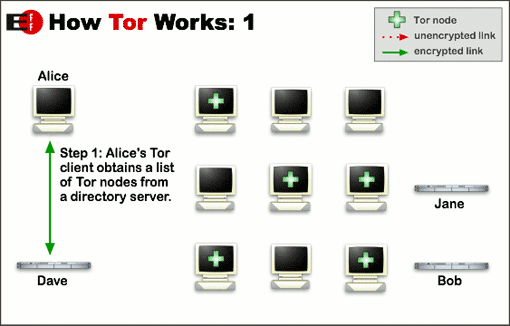
\includegraphics[scale=0.54]{imgs/tor1.png}
\end{center}
\end{frame}

\begin{frame}{Tor}{Tor workings}
\begin{center}
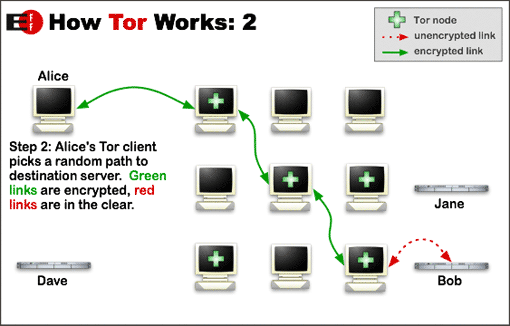
\includegraphics[scale=0.54]{imgs/tor2.png}
\end{center}
\end{frame}

\begin{frame}{Tor}{Tor workings}
\begin{center}
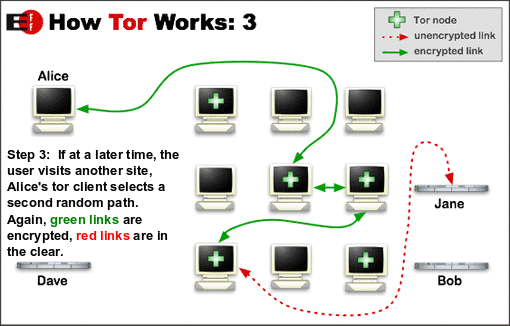
\includegraphics[scale=0.72]{imgs/tor3.png}
\end{center}
\end{frame}

\begin{frame}{Tor}{Tor encryption}
\begin{center}
	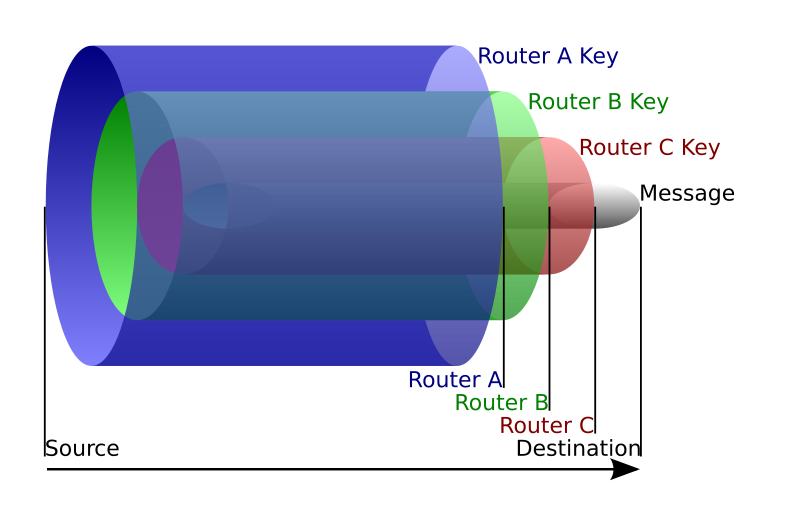
\includegraphics[scale=0.35]{imgs/onion.png}
\end{center}
\end{frame}

\begin{frame}{Tor}{Tor Hidden Service}
\begin{center}
	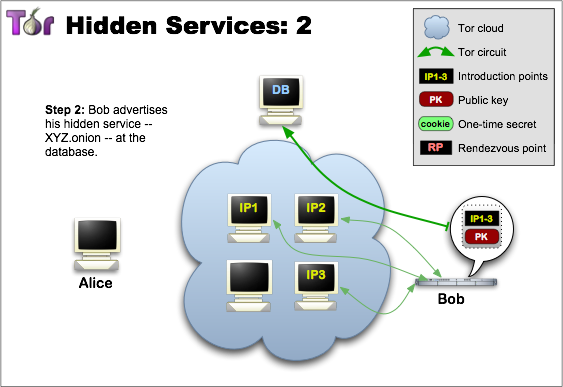
\includegraphics[scale=0.45]{imgs/THS-2.png}
\end{center}
\end{frame}

\begin{frame}{Tor}{Tor Hidden Service}
\begin{center}
	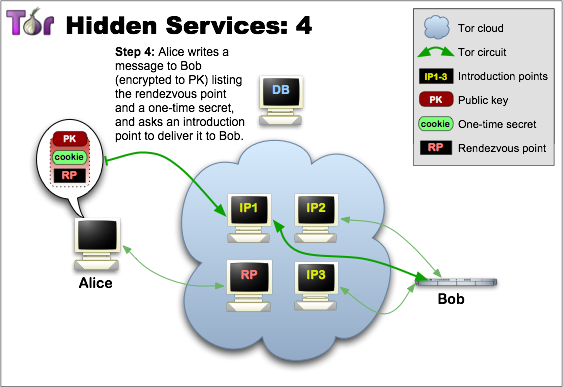
\includegraphics[scale=0.45]{imgs/THS-4.png}
\end{center}
\end{frame}

\begin{frame}{Tor}{Tor Hidden Service}
\begin{center}
	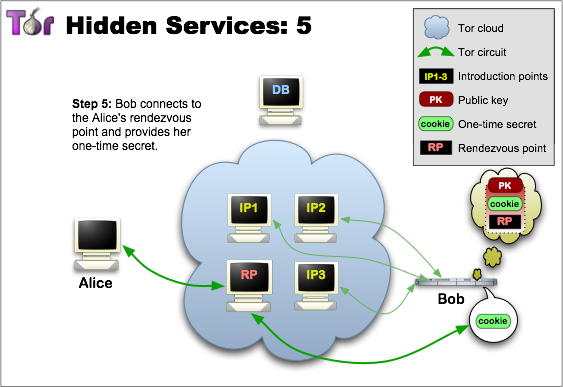
\includegraphics[scale=0.45]{imgs/THS-5.png}
\end{center}
\end{frame}

\begin{frame}{Tor}{Tor Hidden Service}
\begin{center}
	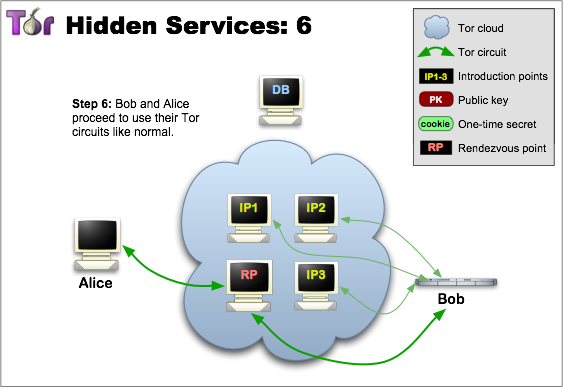
\includegraphics[scale=0.45]{imgs/THS-6.png}
\end{center}
\end{frame}

\begin{frame}{Tor}{Summary}
\begin{center}
	\begin{itemize}
		\item Base: anonymity of clients
		\item Hidden services: anonymity of client + anonymity of servers
	\end{itemize}
	
	\begin{center}
			\large{\emph{But ... is it enough?''}}
	\end{center}

\end{center}
\end{frame}
